% Options for packages loaded elsewhere
\PassOptionsToPackage{unicode}{hyperref}
\PassOptionsToPackage{hyphens}{url}
%
\documentclass[
  ignorenonframetext,
]{beamer}
\usepackage{pgfpages}
\setbeamertemplate{caption}[numbered]
\setbeamertemplate{caption label separator}{: }
\setbeamercolor{caption name}{fg=normal text.fg}
\beamertemplatenavigationsymbolsempty
% Prevent slide breaks in the middle of a paragraph
\widowpenalties 1 10000
\raggedbottom
\setbeamertemplate{part page}{
  \centering
  \begin{beamercolorbox}[sep=16pt,center]{part title}
    \usebeamerfont{part title}\insertpart\par
  \end{beamercolorbox}
}
\setbeamertemplate{section page}{
  \centering
  \begin{beamercolorbox}[sep=12pt,center]{part title}
    \usebeamerfont{section title}\insertsection\par
  \end{beamercolorbox}
}
\setbeamertemplate{subsection page}{
  \centering
  \begin{beamercolorbox}[sep=8pt,center]{part title}
    \usebeamerfont{subsection title}\insertsubsection\par
  \end{beamercolorbox}
}
\AtBeginPart{
  \frame{\partpage}
}
\AtBeginSection{
  \ifbibliography
  \else
    \frame{\sectionpage}
  \fi
}
\AtBeginSubsection{
  \frame{\subsectionpage}
}
\usepackage{amsmath,amssymb}
\usepackage{lmodern}
\usepackage{ifxetex,ifluatex}
\ifnum 0\ifxetex 1\fi\ifluatex 1\fi=0 % if pdftex
  \usepackage[T1]{fontenc}
  \usepackage[utf8]{inputenc}
  \usepackage{textcomp} % provide euro and other symbols
\else % if luatex or xetex
  \usepackage{unicode-math}
  \defaultfontfeatures{Scale=MatchLowercase}
  \defaultfontfeatures[\rmfamily]{Ligatures=TeX,Scale=1}
  \setmainfont[BoldFont = SF Pro Rounded Semibold]{SF Pro Rounded}
  \setmathfont[]{STIX Two Math}
\fi
\usefonttheme{serif} % use mainfont rather than sansfont for slide text
% Use upquote if available, for straight quotes in verbatim environments
\IfFileExists{upquote.sty}{\usepackage{upquote}}{}
\IfFileExists{microtype.sty}{% use microtype if available
  \usepackage[]{microtype}
  \UseMicrotypeSet[protrusion]{basicmath} % disable protrusion for tt fonts
}{}
\makeatletter
\@ifundefined{KOMAClassName}{% if non-KOMA class
  \IfFileExists{parskip.sty}{%
    \usepackage{parskip}
  }{% else
    \setlength{\parindent}{0pt}
    \setlength{\parskip}{6pt plus 2pt minus 1pt}}
}{% if KOMA class
  \KOMAoptions{parskip=half}}
\makeatother
\usepackage{xcolor}
\IfFileExists{xurl.sty}{\usepackage{xurl}}{} % add URL line breaks if available
\IfFileExists{bookmark.sty}{\usepackage{bookmark}}{\usepackage{hyperref}}
\hypersetup{
  pdftitle={444 Lecture 5.2 - Mixed Strategies},
  pdfauthor={Brian Weatherson},
  hidelinks,
  pdfcreator={LaTeX via pandoc}}
\urlstyle{same} % disable monospaced font for URLs
\newif\ifbibliography
\usepackage{graphicx}
\makeatletter
\def\maxwidth{\ifdim\Gin@nat@width>\linewidth\linewidth\else\Gin@nat@width\fi}
\def\maxheight{\ifdim\Gin@nat@height>\textheight\textheight\else\Gin@nat@height\fi}
\makeatother
% Scale images if necessary, so that they will not overflow the page
% margins by default, and it is still possible to overwrite the defaults
% using explicit options in \includegraphics[width, height, ...]{}
\setkeys{Gin}{width=\maxwidth,height=\maxheight,keepaspectratio}
% Set default figure placement to htbp
\makeatletter
\def\fps@figure{htbp}
\makeatother
\setlength{\emergencystretch}{3em} % prevent overfull lines
\providecommand{\tightlist}{%
  \setlength{\itemsep}{0pt}\setlength{\parskip}{0pt}}
\setcounter{secnumdepth}{-\maxdimen} % remove section numbering
\let\Tiny=\tiny

 \setbeamertemplate{navigation symbols}{} 

% \usetheme{Madrid}
 \usetheme[numbering=none, progressbar=foot]{metropolis}
 \usecolortheme{wolverine}
 \usepackage{color}
 \usepackage{MnSymbol}
% \usepackage{movie15}

\usepackage{amssymb}% http://ctan.org/pkg/amssymb
\usepackage{pifont}% http://ctan.org/pkg/pifont
\newcommand{\cmark}{\ding{51}}%
\newcommand{\xmark}{\ding{55}}%

\DeclareSymbolFont{symbolsC}{U}{txsyc}{m}{n}
\DeclareMathSymbol{\boxright}{\mathrel}{symbolsC}{128}
\DeclareMathAlphabet{\mathpzc}{OT1}{pzc}{m}{it}

\setlength{\parskip}{1ex plus 0.5ex minus 0.2ex}

\AtBeginSection[]
{
\begin{frame}
	\Huge{\color{darkblue} \insertsection}
\end{frame}
}

\renewenvironment*{quote}	
	{\list{}{\rightmargin   \leftmargin} \item } 	
	{\endlist }

\definecolor{darkgreen}{rgb}{0,0.7,0}
\definecolor{darkblue}{rgb}{0,0,0.8}

\usepackage[italic]{mathastext}
\usepackage{nicefrac}

\setbeamertemplate{caption}{\raggedright\insertcaption}

%\def\toprule{}
%\def\bottomrule{}
%\def\midrule{}
\usepackage{etoolbox}
\AfterEndEnvironment{description}{\vspace{9pt}}
\AfterEndEnvironment{oltableau}{\vspace{9pt}}
\BeforeBeginEnvironment{oltableau}{\vspace{9pt}}
\AfterEndEnvironment{center}{\vspace{9pt}}
\BeforeBeginEnvironment{tabular}{\vspace{9pt}}
\AfterEndEnvironment{longtable}{\vspace{-6pt}}
\usepackage{booktabs}
\usepackage{longtable}
\usepackage{array}
\usepackage{multirow}
\usepackage{wrapfig}
\usepackage{float}
\usepackage{colortbl}
\usepackage{pdflscape}
\usepackage{tabu}
\usepackage{threeparttable} 
\usepackage{threeparttablex} 
\usepackage[normalem]{ulem} 
\usepackage{makecell}
\usepackage{xcolor}
\usepackage{ulem}

\setlength\heavyrulewidth{0ex}
\setlength\lightrulewidth{0.08ex}

\aboverulesep=0ex
\belowrulesep=0ex
\renewcommand{\arraystretch}{1.2}
\ifluatex
  \usepackage{selnolig}  % disable illegal ligatures
\fi

\title{444 Lecture 5.2 - Mixed Strategies}
\author{Brian Weatherson}
\date{}

\begin{document}
\frame{\titlepage}

\begin{frame}{Plan}
\protect\hypertarget{plan}{}
Introduce the idea of mixed strategies
\end{frame}

\begin{frame}{Reading}
\protect\hypertarget{reading}{}
Bonanno, section 6.2
\end{frame}

\begin{frame}{Core Idea}
\protect\hypertarget{core-idea}{}
Flip a coin!
\end{frame}

\begin{frame}{Motivation}
\protect\hypertarget{motivation}{}
\begin{figure}
\centering
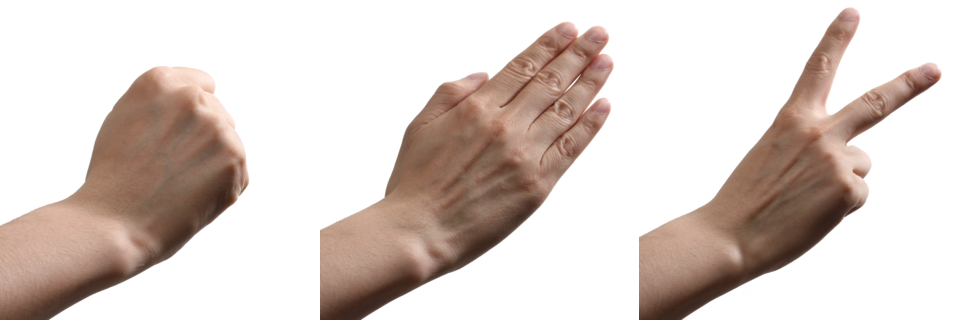
\includegraphics{images/rps.png}
\caption{Rock! Paper!! Scissors!!!}
\end{figure}
\end{frame}

\begin{frame}{Payout}
\protect\hypertarget{payout}{}
If Row plays 60\% Up and 40\% Down, and Column plays Left, then Row's
expected payout will be

\begin{itemize}
\tightlist
\item
  0.6 times the payout for Up/Left
\item
  0.4 times the payout for Down/Left \pause
\end{itemize}

When we evaluate a mixed strategy, we evaluate it by its expected
payout, not its actual payout.
\end{frame}

\begin{frame}{Payout}
\protect\hypertarget{payout-1}{}
If Row plays 60\% Up and 40\% Down, and Column plays Left, then Column's
payout will be

\begin{itemize}
\tightlist
\item
  0.6 times the payout for Left/Up
\item
  0.4 times the payout for Left/Down \pause
\end{itemize}

We have to use expected values for evaluating even \textbf{pure}
strategies like Left, once one player plays mixtures.
\end{frame}

\begin{frame}{Both Mixing}
\protect\hypertarget{both-mixing}{}
What if Column also mixes, playing 70\% Left and 30\% Right.

\begin{itemize}
\tightlist
\item
  Then Row's expected payout is 0.7 times the \textbf{expected} payout
  of their mixed strategy when Column plays Left, plus 0.3 times the
  expected payout of their mixed strategy when Column plays right.
\item
  We have to use expected values twice over to get the philosophically
  important value of this strategy.
\end{itemize}
\end{frame}

\begin{frame}{Independence}
\protect\hypertarget{independence}{}
\begin{itemize}
\tightlist
\item
  What we're assuming here is that the probabilities of each player are
  \textbf{independent}.
\item
  If they roll 20-sided dice or whatever, they roll different ones.
\item
  There is an interesting part of game theory where we drop that
  assumption, but I'm not going to cover it.
\item
  This is the part that deals with so-called \textbf{correlated
  equilibrium}.
\item
  Bonanno doesn't cover this, and I won't either.
\end{itemize}
\end{frame}

\begin{frame}{What is a Mixed Strategy}
\protect\hypertarget{what-is-a-mixed-strategy}{}
At least three interpretations.

\begin{enumerate}
\tightlist
\item
  Random device
\item
  Frequencies
\item
  Epistemic
\end{enumerate}
\end{frame}

\begin{frame}{Random Device}
\protect\hypertarget{random-device}{}
\begin{itemize}
\tightlist
\item
  I mean, you literally roll a die, flip a coin, use something on your
  phone or something.
\item
  This is the traditional interpretation, but it's become less popular.
\end{itemize}
\end{frame}

\begin{frame}{Frequencies}
\protect\hypertarget{frequencies}{}
\begin{itemize}
\tightlist
\item
  In the long-run, your frequency of each play tracks the probabilities
  in the strategy.
\item
  And more specifically, your frequency of each play in each
  identifiable situation tracks the probabilities.
\item
  Alternating rock-then-paper-then-scissors isn't a way to play the
  mixed strategy 1/3 for each move.
\item
  Relatedly, you will lose.
\item
  On the frequency interpretation of mixed strategies, playing that
  mixed strategy means that after rock, you'll play 1/3 rock, 1/3 paper,
  1/3 scissors, and after paper-then-scissors, you'll play \ldots, and
  so on.
\end{itemize}
\end{frame}

\begin{frame}{Epistemic}
\protect\hypertarget{epistemic}{}
\begin{itemize}
\tightlist
\item
  A rational onlooker will not be able to figure out what you will
  do/are doing, beyond saying that you're playing each strategy with the
  specified probability.
\item
  It doesn't matter how you get there, as long as that's all that an
  onlooker (or co-player) can figure out.
\end{itemize}
\end{frame}

\begin{frame}{Mixtures Always Available}
\protect\hypertarget{mixtures-always-available}{}
\begin{itemize}
\tightlist
\item
  Game theorists standardly assume that if some moves are available, so
  is any mixed strategy built out of them.
\item
  Philosophers do not assume this, and often think it's the least
  plausible thing about game theory.
\item
  Is this assume plausible?
\end{itemize}
\end{frame}

\begin{frame}{What's a Mixed Theory}
\protect\hypertarget{whats-a-mixed-theory}{}
\begin{itemize}
\tightlist
\item
  On the random device interpretation, it's very implausible.
\item
  Not all game players have arbitrary random devices available.
\item
  But on the other interpretations, it is more plausible.
\item
  A good player should be able to hide their strategy, even in repeated
  plays.
\end{itemize}
\end{frame}

\begin{frame}{For Next Time}
\protect\hypertarget{for-next-time}{}
We will look at a striking consequence of the existence of mixed
strategies - every game has a Nash equilibrium.
\end{frame}

\end{document}
